\subsection{1D Exact}

% \begin{frame}{1D: Encodings + Error Measure}
%     % \begin{minipage}{.6\textwidth}

%     % \end{minipage}
%     % \begin{minipage}{.39\textwidth}

%     %     \begin{table}[]
%     %         \caption*{$\chi$}
%     %         \begin{tabular}{l l|l l }
%     %                                                    &   & \multicolumn{2}{c}{Encoding}       \\
%     %                                                    &   & A                            & E/F \\
%     %             \hline
%     %             \multirow{3}{*}{\rotatebox{90}{Order}} & 3 & 5                            & 10  \\
%     %                                                    & 5 & 21                           & 42  \\
%     %                                                    & 7 & 85                           & 170 \\
%     %         \end{tabular}
%     %     \end{table}
%     % \end{minipage}
% \end{frame}

\begin{frame}{1D: Transverse Field Ising (TFI) }

    \begin{minipage}{.6\textwidth}
        \begin{figure}
            \center
            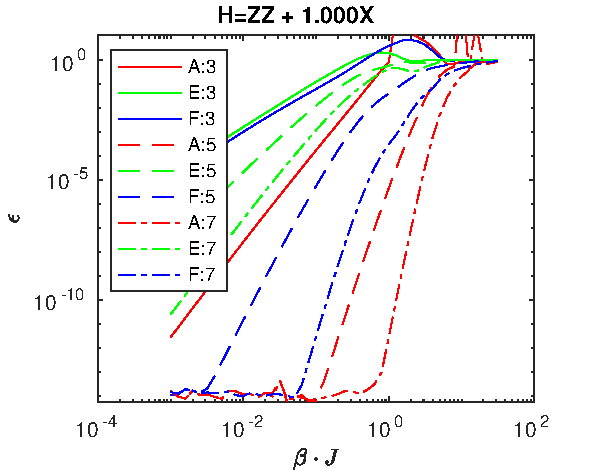
\includegraphics[height=0.9\textheight]{../Figuren/benchmarking/t_ising_small.pdf}
        \end{figure}
    \end{minipage}
    \begin{minipage}{.39\textwidth}

        \begin{itemize}
            \item Relative error $\epsilon$
            \item Different encodings:
                  \begin{itemize}
                      \item A: Small
                      \item E: Strict
                      \item F: well-conditioned
                  \end{itemize}

            \item bond dimension

                  \begin{table}[]
                      %\caption*{$\chi$}
                      \begin{tabular}{l l|l l }
                                                                 &   & \multicolumn{2}{c}{Encoding}       \\
                                                                 &   & A                            & E/F \\
                          \hline
                          \multirow{3}{*}{\rotatebox{90}{Order}} & 3 & 5                            & 10  \\
                                                                 & 5 & 21                           & 42  \\
                                                                 & 7 & 85                           & 170 \\
                      \end{tabular}
                  \end{table}

        \end{itemize}
    \end{minipage}

\end{frame}

\begin{frame}{Conclusion}
    \begin{itemize}
        \item Large $\beta$-steps
        \item Real time evolution
        \item Encoding
        \item Truncation $\chi$
    \end{itemize}
\end{frame}

\subsection{TFI Phase Diagram}

\begin{frame}{2D TFI: Introduction}
    \begin{minipage}{0.35\textwidth}
        \begin{itemize}
            \item Phase Transition
            \item Criticality
            \item Finite size scaling
                  \begin{itemize}
                      \item Observables:

                            $m$, $S$ and $\xi$
                      \item Parameters:

                            $T_c$, exponents
                  \end{itemize}
            \item $\Gamma=2.5$
            \item VUMPS ($\chi$,$\delta^{-1}$)
        \end{itemize}
    \end{minipage}
    \begin{minipage}{0.64\textwidth}
        \begin{figure}
            \centering
            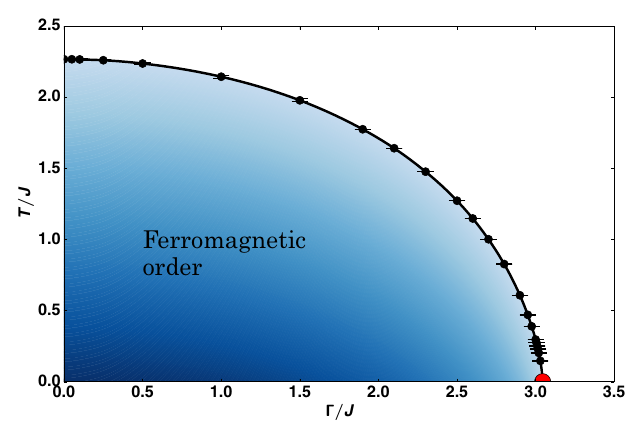
\includegraphics[width=\linewidth]{../Figuren/phsyics/2disingphase.png}
            \caption*{Figure taken from \cite{Hesselmann2016}  }
        \end{figure}
    \end{minipage}
\end{frame}

\begin{frame}{TFI Phase Diagram: $\Gamma=2.5$}
    \begin{minipage}{.75\textwidth}
        \begin{figure}
            \center
            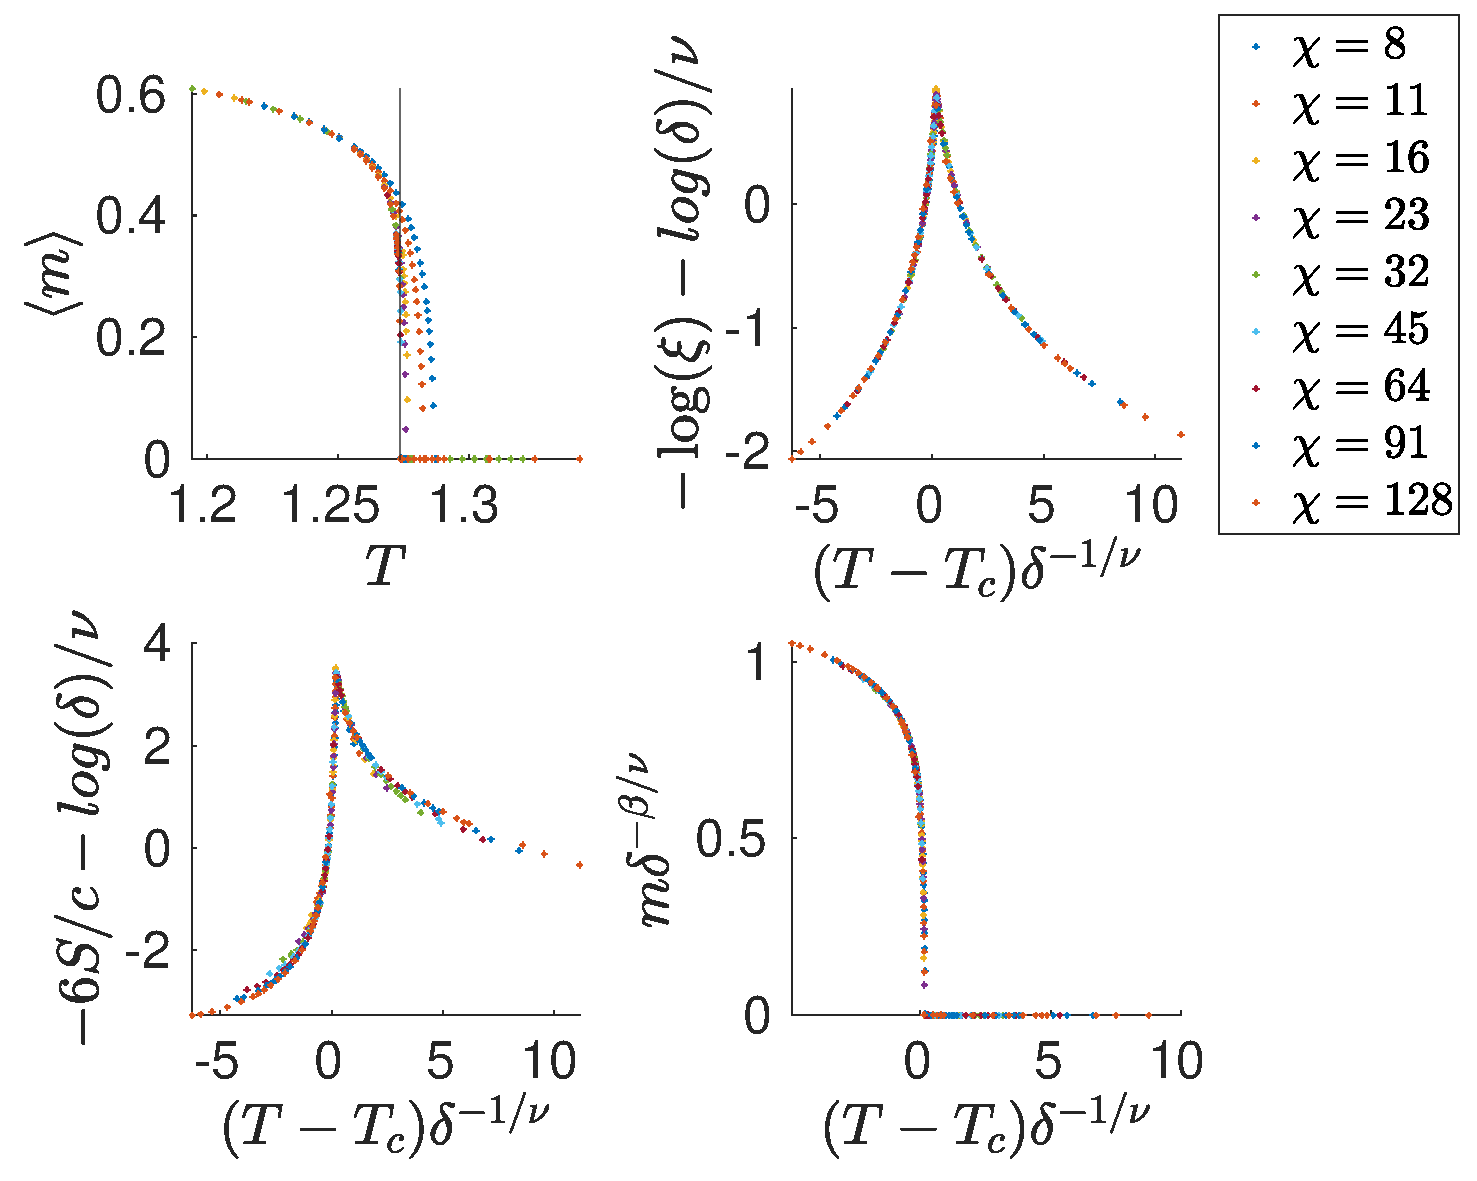
\includegraphics[height=\textheight]{../Figuren/phasediag/g25/zoomed_small.pdf}
        \end{figure}
    \end{minipage}
    \begin{minipage}{.24\textwidth}
        \begin{table}[]

            \begin{tabular}{l|l }
                    & $T_c$     \\
                \hline          \\
                Fit & 1.2736(6) \\
                QMC & 1.2737(6) \\
                TN  & 1.2737(2) \\
            \end{tabular}
            \caption*{Data from  \cite{Czarnik2019} }
        \end{table}
    \end{minipage}
\end{frame}

